\documentclass[10pt,paper=a4,final]{scrartcl}
\usepackage[utf8]{inputenc}
\usepackage{tabularx}		%used for the tables
\usepackage{geometry}		%allows us to specify the 'seitenrand'
\usepackage[table]{xcolor}	%allows us to make colored fields in the tables
\usepackage{graphicx}		%package used to include graphics
\usepackage{hyperref}   	%used to make klickable links

%\hypersetup{linktocpage}	%make the tableofcontent klickable
\hypersetup{
  colorlinks,
  citecolor=black,
  filecolor=black,
  linkcolor=black,
  urlcolor=black
}

\setcounter{tocdepth}{4}	%include paragraph in tableofcontents
\setcounter{secnumdepth}{5}	%also number the paragraphs

%These two lines will allow us to specify our own headers/footers
\usepackage{fancyhdr}
\pagestyle{fancy}
 \setlength{\parskip}{0pt}
 \setlength{\baselineskip}{0pt}

%The next three lines set the default font to Arial
%use 'getnonfreefonts arial-urw' to install uarial on Linux systems
\usepackage[T1]{fontenc}
\usepackage[scaled]{uarial}
\renewcommand*\familydefault{\sfdefault}

\geometry{a4paper, top=20mm, right=20mm, bottom=20mm, left=20mm}
\title{Realisierungsbericht}
\author{Niklaus Hofer, Lukas Kn\"opfel, Kaleb Tschabold}
\date{\today}

%defining header and footer
\fancyhf{}	%delete default values
\setlength{\headwidth}{\textwidth}	%header and footer width equal the text width
\fancyhead[LE,LO]{
\includegraphics[scale=0.6]{header.png}}
\fancyhead[RE,RO]{ProjectExplorer}
\fancyfoot[CE,CO]{Speicherdatum: \today{}}
\fancyfoot[RE,RO]{\thepage}

\begin{document}
\maketitle
\newpage
\begin{tabularx}{\textwidth}{ r X }	%X fields are stretched over the whole space
  \textcolor{white}{{\bf Status}}\cellcolor{blue!80!} & In Arbeit/{\bf In Prüfung}/ Abgeschlossen\cellcolor{blue!20!} \\
\textcolor{white}{{\bf Projektname}}\cellcolor{blue!80!} & Projektexplorer\cellcolor{blue!20!} \\
\textcolor{white}{{\bf Projektleiter}}\cellcolor{blue!80!} & Lukas Kn\"opfel\cellcolor{blue!20!} \\
\textcolor{white}{{\bf Auftraggeber}}\cellcolor{blue!80!} & M. Frieden, GIBB\cellcolor{blue!20!} \\
\textcolor{white}{{\bf Autoren}}\cellcolor{blue!80!} & Kaleb Tschabold, Lukas Kn\"opfel, Niklaus Hofer\cellcolor{blue!20!} \\
\textcolor{white}{{\bf Verteiler}}\cellcolor{blue!80!} & Lukas Knöpfel, Kaleb Tschabolt, Niklaus Hofer\cellcolor{blue!20!}
\end{tabularx}
\newline
\newline
\newline
{\bf Änderungskontrolle, Prüfung, Genehmigung}
\newline

\begin{tabularx}{\textwidth}{l l X X}
\textcolor{white}{Version}\cellcolor{blue!80!} & \textcolor{white}{Datum}\cellcolor{blue!80!} & \textcolor{white}{Beschreibung, Bemerkung}\cellcolor{blue!80!} & \textcolor{white}{Name oder Rolle}\cellcolor{blue!80!} \\
\cellcolor{blue!20!} 0.1& \cellcolor{blue!20!} 08.02.2011 & Gesammelten Text einfügen \cellcolor{blue!20!} & Kaleb Tschabold \cellcolor{blue!20!} \\
\cellcolor{blue!20!} 0.9& \cellcolor{blue!20!} 08.02.2011 & Abgabebereit \cellcolor{blue!20!} & Kaleb Tschabold \cellcolor{blue!20!} \\
\cellcolor{blue!20!} 0.99& \cellcolor{blue!20!} \today{} & Transfer nach \LaTeX \cellcolor{blue!20!} & Niklaus Hofer \cellcolor{blue!20!} \\
\cellcolor{blue!20!} 1.0& \cellcolor{blue!20!} \today{} & Korrekturen \cellcolor{blue!20!} & Niklaus Hofer \cellcolor{blue!20!} \\
\end{tabularx}
\newline
\newline
\newline
{\bf Definitionen und Abkürzungen}
\newline

\begin{tabularx}{\textwidth}{l X}
\textcolor{white}{Begriff/ Abkürzung}\cellcolor{blue!80!} & \textcolor{white}{Bedeutung}\cellcolor{blue!80!} \\
CLI \cellcolor{blue!20!} & Command Line Interface\cellcolor{blue!20!} \\
\end{tabularx}
\newline
\newline
\newline
\bibliographystyle{plain}
\bibliography{projektantrag}{}
\flushleft
\newpage
\tableofcontents
\newpage
\section{Zweck des Dokuments}
Wir hatte jetzt einige Wochen Zeit um an der Realisierungs zu arbeiten. Wir konnten jetzt unsere Programm Spezifikationen noch genauer ausarbeiten, weil wir während dem programmieren gesehen haben was noch verbessert oder ergänzt werden sollte. In diesem Dokumente sind jetzt die genauen Informationen zum Programm.
\section{Technische Detailspezifikation}
\subsection{Innere Struktur}
\subsubsection{L\"osungsvorschl\"age f\"ur die Struktur des Systemdesigns}
Es gibt zwei wichtige Entscheidungen zum Systemdesign, die w\"ahrend der Realisierung getroffen wurden.\\
Die Erste betrifft, das GUI, die zweite die Art wie die Daten in der Datenbank abgelegt werden.
\paragraph{GUI}
Die \"Anderung am GUI betrifft die Art und Weise wie die Tags zu den Dateien zugeordnet werden. Unser erster Einfall dazu war der, dass sich \"uber das Kontextmen\"u der Dateien ein Popup \"offnen liesse, in dem die Tags zugeordnet werde k\"onnten.\\
F\"ur ein Programm, dessen Hauptaufgabe gerade die Verwaltung der Tags darstellt, ist diese Art Tags Dateien zu zu ordnen aber recht aufwendig.

Die Verwaltung der Tags wird nun unabh\"angig von der Ansicht (Tag oder Hierarchisch) immer auf der rechten Seite des Programms angezeigt. Sobald in der linken Spalte eine Datei angew\"ahlt wird, werden deren Tags in der rechten aufgelistet.\\
Zudem k\"onnen der Datein von dort aus weitere, bereits bestehende, Tags per Doppelklick zugeordnet oder ganz neue hinzugef\"ugt werden, indem man deren Namen, Komma getrennt, der Liste der Tags anh\"angt.

Diese L\"osung, f\"ur die wir uns entschieden haben ist weniger umst\"andlich und macht die Aufgabe des Programms gleich beim Start deutlich.
\paragraph{Datenstruktur}
Die zweite wichtige Entscheidung betrifft die Art, wie die Pfade zu den Dateien in der Datenbank abgelegt werden.\\
Damit Dateien anhand ihrer URI in der Datenbank gefunden werden k\"onnen muss die Art, wie die URI abgelegt wird immer gleich sein.\\
Aus Datenbank-technischer Sicht ist es von Vorteil, den Pfad zur Datei vom Dateinamen getrennt zu speichern. Abfragen nach ‘allen Dateien aus dem Verzeichnis X’ werden so deutlich einfacher aus zu f\"uhren.\\
Auch beim Darstellen der Dateien ist diese Art des Speicherns meist von Vorteil, da der Dateiname immer getrennt vom Pfad dargestellt wird (der Pfad oben, wie von Windows Explorer gew\"ohnt, und der Dateinamen unten im mittleren Panel).\\
Diese getrennt Speicherung hat aber zu der Frage gef\"uhrt ob / (oder \ in Windows) am Ende der Pfadangabe mitgespeichert werden solle.\\
Wir entschieden uns daf\"ur, damit Pfade ohne weiteren Aufwand vollst\"andig zusammengesetzt werden k\"onnen.\\
Ist der ‘Dateinamen’ der Name eines neuen Verzeichnisses, so tr\"agt auch er ein / (oder \ in Windows) am Ende.
\subsubsection{Struktur des Systemdesigns}
\subsubsection{Beschreibung der Elemente}
\begin{description}
  \item{\bf Main} Wird zum Starten des Programmes aufgerufen. Main.py instanziert alle weiteren Elemente die f\"ur das Funktionieren des Programms n\"otig sind und koordiniert die Kommunikation zwischen den einzelnen Elementen.
  \item{\bf DB} DB.py ist ein interface zur Datenbank. Es nimmt allen anderen Klassen die Aufgabe ab selbst SQL statements ab zu setzen und bietet stattdessen nach aussen hin verschiedene Funktionen an um Daten zu lesen oder zu schreiben.
  \item{\bf Utility} Enth\"alt verschiedene n\"utzliche Methoden die immer mal wieder von einzelnen Teilen des Programmes ben\"otigt werden.
  \item{\bf CLI} Dient als Command-line-interface f\"ur das Program. Es nimm \"uber die Kommandozeile beim Aufruf verschiedene Befehle entgegen die es dann asf\"uhrt.
  \item{\bf TagManager} Der Tag Manger ist für kleine Tag Verwaltungsaufgaben zuständig.
  \item{\bf FileManager} Über den FileManager wird auf das Dateisystem zugegriffen. Hier wird aus jeder Datei aus dem File System ein File Objekt erstellt.
  \item{\bf FileSystemListener} Registriert beim Kernel Listener f\"ur zu \"uberwachende Ordner. Wird in diesen Ordnern eine Operation ausgef\"uhrt (wie das Verschieben, L\"oschen, Umbenennen oder Erstellen einer Datei), so wird der FileSystemListener vom Kernel dar\"uber in Kenntnis gesetzt, woraufhin er wiederum die n\"otigen Aktionen ausl\"ost um die Datenbank auf dem aktuellen Stand zu halten.\\
    Dies soll dazu beitragen, dass m\"oglichst selten Dateien angezeigt werden, die auf Dateisystem-Ebene nicht existieren.
  \item{\bf GUI} Ist f\"ur die grafische Darstellung des Programms mittels GTK zust\"andig. Das GUI ist in der Lage je nach Bedarf eine andere ‘View’ darzustellen. Direkt nach dem Programmstart wird HierachicalView dargestellt. Im Betrieb kann jederzeit zwischen ‘TagView’ und ‘HirachicalView’ umgeschaltet werden.\\
    Dazu kann GUI, per Polymorphismus, eine Klasse aufnehmen die von ‘View’ erbt.
  \item{\bf TagView} Enth\"alt die Darstellung der Tag-Ansicht und wird von ‘GUI’ bei Bedarf geladen.
  \item{\bf HierarchicalView} Enth\"alt die Darstellung der hierachischen Ansicht und wird von ‘GUI’ bei Bedarf geladen.
  \item{\bf View} Mutterklasse von GUI.
  \item{\bf File} Repr\"asentiert eine Datei und wird benutzt um Iformationen \"ueber Dateine zwischen den Elementen des Programms auszutauschen. Fuer mehr Informationen siehe 2.3.2.
\end{description}
\subsection{Schnittstellendefinition}
\begin{enumerate}
\item Interne Schnittstellen
\begin{enumerate}
\item Intern ist die Kommunikation mit der Datenbank sehr wichtig.
\begin{enumerate}
\item Die Datenbank-Schnittstelle ist in DB.py implementiert.
\item Die Schnittstelle nimmt in den meisten F\"allen Objekte vom Typ File(.py). In anderen auch Strings.
\item Welche Funktionen in der Schnittstelle genau definiert sind, kann dem Klassendiagramm entnommen werden.\\
Wie die einzelnen Methoden aufzurufen sind und was sie genau tun kann, ist jeweils im Methodenkommentar ersichtlich.
\end{enumerate}
\end{enumerate}
\item Externe Schnittstellen
\begin{enumerate}
\item Für den normalen Gebrauch haben wie das GUI. Beim GUI wird Wert auf das einfache verwalten von Tags und Dateien gelegt.
\begin{enumerate}
\item Das GUI bietet zwei Modi, einer der den herkömlichen Dateimanagern mit hierarchischer Ansicht entspricht und
\item Einen Tagmodus, in dem sich Dateien anhand deren Tags durchsuchen und ordnen lassen.
\end{enumerate}
\item Für scripting oder für solche Systeme ohne grafische Ausgabe haben wir eine CLI Version. Es wird besonders Wert auf das einfache Aufrufen von anderen Programmen (Scripts) gelegt. (nicht implementiert)
\begin{enumerate}
\item Die Kommandos sollen in der Bedienung weitgehend mit dem standard Unix-Tools kompatibel
\end{enumerate}
\end{enumerate}
\end{enumerate}
\subsection{Datenmodell}
\subsubsection{Datenbank}
\begin{figure}[h!]
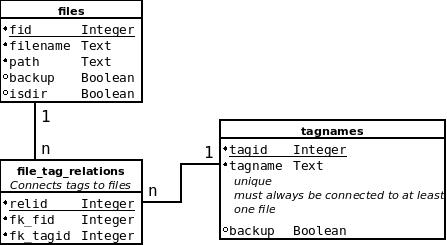
\includegraphics[scale=1.0]{db.jpeg}
\caption{Datenbankschema}
\end{figure}
Die Datenbank l\"asst sich \"uber DB.py ansprechen, siehe Schnittstellendefinition f\"ur mehr Informationen.\\
Welche Felder genau welche Information enthalten ist eim folgenden Abschnitt erl\"autert.
\subsubsection{File-object}
Informationen \"uber einzelne Dateien werden innerhalb des Programms mit Hilfe des File objects festgehalten und ausgetauscht.\\
Das File Object hat f\"ur alle Variablen Getter und Setter, sie alle k\"onnen aber auch im Konstruktor angegeben werden.\\
Hier eine Auflistung und erl\"auterung zu den einzelnen Variablen der File Klasse:
\begin{tabularx}{\textwidth}{|l|l|X|X|}
  \hline
  \bf Name & \bf Type & \bf Erl\"auterungen & \bf Entsprechung in der Datenbank \\ \hline
  fileName & String & H\"alt den Namen der Datei. Ist der ‘Name’ der eines Verzeichnisses, so endet er mit / (oder \textbackslash in Windows) & files.filename \\ \hline
  path & String & H\"alt den Pfad zu dem Verzeichnis in dem die Datei liegt. Endet mit / (oder \textbackslash in Windows) & files.path \\ \hline
  isDir & Boolean & Besagt, ob das Objekt eine Datei oder ein Verzeichnis repräsentiert. & files.isdir \\ \hline
  backup & Boolean & Besagt, ob Backups der Datei angelegt werden sollen. & files.backup \\ \hline
  fullPath & String & Der ganze Pfad zur Datei inklusive deren Namen. Wird der Fullpath an ein File object \"ubergeben, so wir dieser mittels Regex zerlegt und die Werte in fileName und path abgelegt. & files.path + files.filename \\ \hline
  tags & list[String] & Ent\"alte eine Liste aller Tags die der Datei zugeordnet sind als Strings. & Die Werte in Tagnames werden mit file\_tag\_relation mit denen in files verkn\"upft. \\ \hline
\end{tabularx}
\subsection{Sicherheit}
Die Datenbank liegt auf dem lokaeln Dateisystem und stellt nach Aussen (\"uber das Netzwerk) keine Schnittstelle zur Verf\"ugung.\\
Fuer jeden Nutzer der Software wird in dessen Home-Verzeichnis (unter Unix also /home/username/) ein Ordner ./project-browser angelegt, in dem sich die Datenbank-Datei befindet.\\
Die Datenbank ist also durch die Zugriffsberechtigung des Dateisystems gesch\"utzt und f\"ugt sich somit natlos in bestehende Sicherheits- und Datenschutzkonzepte ein.
\subsection{Anforderungszuordnung}
\begin{enumerate}
  \item Main
  \item DB
  \item Utility
  \item CLI
  \item TagManager
  \item FileManager
  \item FileSystemListener
  \item GUI
  \item TagView
  \item HierarchicalView
  \item View
  \item File
\end{enumerate}
\begin{tabularx}{\textwidth}{|c|X|c|c|c|c|c|c|c|c|c|c|c|c|}
  \hline
  \bf Nr. & \bf Anforderungen &\bf 1 &\bf 2 &\bf 3 &\bf 4 &\bf 5 &\bf 6 &\bf 7 &\bf 8 &\bf 9 &\bf 10 &\bf 11 &\bf 12 \\ \hline
  1 & Das Programm starten & \cellcolor[gray]{0.7} & & & & & & & & & & & \\ \hline
  2 & GUI vorhanden & & & & & & & & \cellcolor[gray]{0.7} &\cellcolor[gray]{0.7} &\cellcolor[gray]{0.7} &\cellcolor[gray]{0.7} & \\ \hline
  3 & CLI vorhanden & & & &\cellcolor[gray]{0.7} & & & & & & & & \\ \hline
  4 & Tag hinzuf\"ugen & & & &\cellcolor[gray]{0.7} &\cellcolor[gray]{0.7} & & & &\cellcolor[gray]{0.7} & & & \\ \hline
  5 & Datei ausw\"ahlen & & & & & & \cellcolor[gray]{0.7} & & & & & & \cellcolor[gray]{0.7} \\ \hline
  6 & Versionierung & & \cellcolor[gray]{0.7} & & & & \cellcolor[gray]{0.7} & \cellcolor[gray]{0.7} & & & & & \cellcolor[gray]{0.7} \\ \hline
  7 & GUI: Versionierung f\"ur Tags & & & & & & & & \cellcolor[gray]{0.7} & & & & \\ \hline
  8 & Datei\"anderungen werden erkannt & & & & & & & & \cellcolor[gray]{0.7} & & & & \\ \hline
  9 & L\"oschen wird erkannt & & & & & & & & \cellcolor[gray]{0.7} & & & & \\ \hline
  10 & Neue Dateien werden erkannt & & & & & & & & \cellcolor[gray]{0.7} & & & & \\ \hline
  11 & Hierarchische Anzeige & & & & & & & & & & & \cellcolor[gray]{0.7} & \\ \hline
  12 & Tag Anzeige & & & & & & & & & \cellcolor[gray]{0.7} & & & \\ \hline
\end{tabularx}
\section{Systemdokumentation}
\subsection{Inline-Dokumentation}
\subsection{Benutzerhandbuch}
\subsubsection{System\"ubersicht}
\paragraph{Aufgabengebiet des Programms}
Das Programm Project-Explorer ist dazu da bei der Verwaltung von Dateien zu helfen.\\
In einer gew\"ohnlichen Arbeitsumgebung werden Dateien in einem hierarchischen System aus Ordnern abgelegt. Doch mit der Datenmenge steigt auch die Komplexit\"at dieser hierarchischen Strukturen und besonders Dateien die selten verwendet werden k\"onnen schwierig aufzufinden sein.\\
Programme zum Verwalten von Musik- und Bilddateien bieten deshalb schon seit vielen Jahren zus\"atzlich sogenannte Metadaten an, um weitere Informationen zu der Datei (z.B. Album, Artist, Aufnahmejahr, … bei Musikdateien) zu speichern mit deren Hilfe sich diese dann einfacher wiederfinden lassen.\\
Projekt-Explorer hat das Ziel \"ahnliches anzubieten - aber nicht auf eine Art von Dateien beschr\"ankt, sonder f\"ur jede Datei, die auf dem lokalen Rechner liegt.\\
Der Nutzer kann dazu den einzelnen Dateien Tags zuordnen, anhand derer er die Dateien sp\"ater wieder finden kann.\\
Die Tags k\"onnen selbst festgelegt und vergeben werden.
\paragraph{Programmoberfl\"ache}
\begin{figure}[h!]
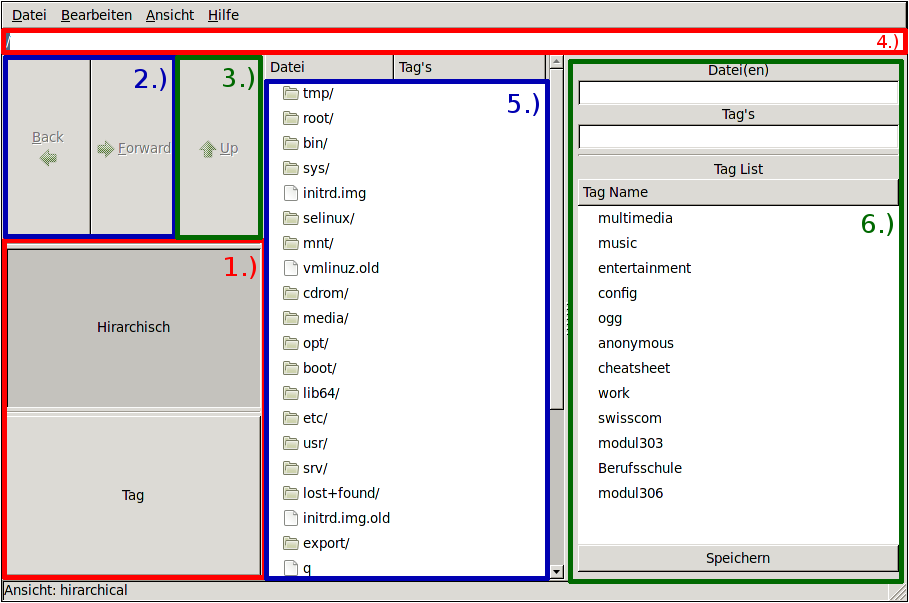
\includegraphics[scale=0.5]{erlaeuterungen_gui.png}
\end{figure}
Die Oberfl\"ache des Programms l\"asst sich grob in vier Bereiche aufteilen.\\
Der Erste (4. auf dem Bild), ist die Multibar. Hier kann der Pfad zu einem Verzeichnis eingeben werden, oder, in der Tag-Ansicht, ein Tag nachdem man sucht.\\
Der Zweite Bereich (1.,2. und 3. auf dem Bild) ist der Navigationsbereich. Hier kann in der Ordnerstruktur navigiertt und zwischen den Ansichten umgeschaltet werden Im dritten Bereich (5. auf dem Bild), werden die Dateien angezeigt. Rechts der Dateien sind deren Tags zu sehen.\\
Der letzte Bereich (6. auf dem Bild) ist der wichtigste. Hier werden die verf\"ugbaren Tags angezeigt und hier k\"onnen die Tags den Dateien zugeordnet werden.\\
\paragraph{Anmerkungen zur korrekten Verwendung unter dem Aspekt der Sicherheit}
Den Autoren ist es wichtig an dieser Stelle einige Bemerkungen zur Datensicherheit zu machen.
Grunds\"atzlich gilt f\"ur die Daten die im Projekt-Explorer erfasst werden dasselbe wie f\"ur alle anderen Daten auf dem Computer auch. Die Informationen werden in einem pers\"onlichen Verzeichnis des Nutzers abgelegt.\\
Per Standard ist dieses vor dem Zugriff durch andere Benutzer gesch\"utzt. Es kann aber in einzelnen F\"allen sein, dass diese Einstellung vom Systemadmnistrator ver\"andert worden ist.
Es ist zudem zu beachten, dass der Systemadministrator zu jeder Zeit Zugriff auf die Daten hat.
Werden im Program sehr pers\"onliche Informatione abgelegt oder handelt es sich beim verwendeten Ger\"at um einen portablen Computer (Ein Laptop oder gar ein Handset) so sollte die lokale Festplatte verschl\"usselt werden, damit im Falle eines Verlustes des Ger\"ates kein unberechtigeter Zugriff auf die Dateien geschehen kann.
\subsubsection{Anwenderfunktionalit\"at}
In dieser Kategorie werden wir einige typische Anwendungen f\"ur Projekt-Explorer beschreiben. Die Erl\"auterungen werden sich zumeiste auf das Bild im Abschnitt ‘Programmoberfl\"ache’ beziehen. Nummern aus dem Bild werden im Format \#1.) angegeben.
Wir werden folgende Szenarien beschreiben:
\begin{itemize}
  \item Wechseln der Ansicht zwischen Tag- und Hierarchischer Ansicht.
  \item Wechseln in ein anderes Verzeichnis und Nutzen der Autovervollst\"andigung.
  \item Navigieren in der History.
  \item \"Offnen von Dateien.
  \item Tags zu Dateien zuordnen.
  \item Tags von Dateien entfernen.
  \item Dateien eines Tags anzeigen.
  \item Fehlermeldungen
\end{itemize}
\paragraph{Ansicht wechseln}
Projekt-Explorer hat zwei verschiedene Ansichten, n\"amlich ‘Hierarchisch’ und ‘Tags’. Beim Wechseln zwischen den Ansichten \"andert sich die Ansicht \#5.).\\
Die Ansicht kann entweder \"ueber die grossen Kn\"opfe in \#1.) gewechselt werden oder in der Men\"uleiste unter dem Punkt “Ansicht".
\paragraph{Verzeichnis wechseln}
Um in der hierarchischen Ansicht das Verzeichnis zu wechseln, gibt man das gew\"unschte Zielverzeichnis in \#4.) ein. W\"ahrend der Eingabe erschein ein Drop-Down mit Verzeichnisvorschl\"agen das w\"ahrend des Tippens laufen aktualisiert wird. In diesem Drop-Down kann ein Verzeichnis mittels der Pfeiltasten auf der Tastatur und Enter, oder mit der Maus ausgew\"ahlt werden.\\
Um in das Verzeichnis oberhalt zu wechseln, kann der Knopf “UP" in \#3.) geklickt werden. Um in ein Unterverzeichnis zu \"offnen, f\"urht man einen Doppelklick auf den entsprchenden Eintrag in \#5.) aus.
\paragraph{Hisotry}
Projekt-Explorer merkt sich in welchem Verzeichnis man zuletzt war. Diese Werte werden zur Laufzeit in der History gespeichert. \"Uber die Buttons “Back" und “Forward" kann in dieser History navigiert werden.\\
Die History von Projekt-Explorer entspricht vom Konzept her ziemlich genau der entsprechenden Funktionalit\"at von Webbrowsern.\\
Beim Schliessen der Applikation geht die History verloren.
\paragraph{Dateien \"Offnen}
Dateien werden durch einen Doppelklick ge\"offnet. Sie werden mit dem Program ge\"offnet, das auf dem Betriebssystem als Standardapplikation f\"r den entsprechenden Dateityp festgelegt ist. Ist f\"ur den Dateityp keine Standard-Applikation festgelegt, so kann die Datei auch nicht ge\"offnet werden.\\
Wichtig! Klickt man in der Tagview auf einen Ordner, so wechselt die Ansicht automatisch zur hierarchischen Ansicht zur\"uck.
\paragraph{Tags hinzuf\"ugen}
Um einer Datei Tags hinzu zu f\"ugen muss diese erst in \#5.) angew\"ahlt werden. Das geschieht \"ueber einmaliges Klicken auf die Datei. Anschliessend werden in \#6.) Informationen zu der Datei angezeigt.\\
Im oberen Feld der Name, im unteren Feld die Tags. Die einzelnen Tags sind jeweils durch ein Komma (“,") getrennt.\\
Im unteren Bereich von \#6.) sind alle bereits verwendeten Tags ersichtlich. Um der Datei eines dieser Tags hinzu zu f\"ugen, doppelklickt man den Eintrag, worfaufhin dieser in der Liste oben erscheint. Alternativ dazu, kann das Tag auch von Hand in der Liste geschrieben werden.\\
Um die \"Anderung zu \"ubernehmen klickt man auf den Knopf ‘speichern’, der sich ganz unten in \#6.) befindet.\\
Will man einen g\"anzlich neuen Tag anf\"ugen, so muss dieser von Hand in die Liste der Tags geschrieben werden. Nat\"urlich muss er durch ein Komma von den anderen Tags getrennt sein.
Nach dem speichern, erscheint der neue Tag auch in der Liste unten.\\
Wichtig! Es k\"onnen keine Tags bestehen, die keiner Datei zugeordnet sind!
\paragraph{Tags entfernen}
Um ein Tag von einer Datei zu entfernen, l\"oscht man den Eitrag aus der Liste ‘Tags’ in \#6.) und dr\"uckt speichern.\\
Ist der Tag mit keiner weiteren Datei verbunden, so verschwindet er aus der \"Auswahlliste in \#6.).
\paragraph{Dateien anhand der Tags durchsuchen}
Um Dateien eines Tags anzuzeigen wechselt man erst in die Tagview. Alle Tags werden dort \"ubereinander angezeigt. Durch das Doppelklicken eines Eintrages werden alle Dateien dieses Tags sichtbar.\\
Alternativ kann der Tagname auch in \#4.) eingegeben werden. W\"ahrend der Eingabe werden Tags vorgeschlagen, die gleich geschrieben werden und im Drop-Down zur Auswahl gestellt.
\paragraph{Fehlermeldungen}
Im Normalbetrieb werden keine Fehlermeldungen ausgegeben. Um Trotzdem Informationen zu auftretenden Fehlern zu erhalten muss das Programm aus dem Terminal gestartet werden. Auftretende Fehler werden dann dort ausgegeben.
\subsection{Supporthandbuch}
\subsubsection{Massnahmen bei Benutzerproblemen}
\begin{itemize}
  \item Die Aufgabenstellung von Projekt-Explorer ist lediglich die Verwaltung der Tags. Obwohl im Programm selbst sehr wohl Dateien angezeigt werden, k\"onnen dateien weder mit copy ‘nd paste noch per drag ‘nd drop in den Ordnern bewegt werden. Das Programm selbst bietet auch keine M\"oglichkeit zum Umbenennen oder L\"oschen von Dateien.
  \item Es ist darauf zu achten, dass die Gr\"osse der beiden rechten Pannels von Projekt-Explorer frei verstellbar ist, indem man die ‘Trennlinie’ mit der Maus weiter nach links oder rechts verschiebt. Schiebt man diese Linie zu weit in die eine Richtung kann es vorkommen, dass eine der Spalten komplett verschwindet. Das l\"asst sich ganz einfach beheben, indem man die Linie wieder verschiebt.
  \item Klickt man einen der Buttons zum Umschalten der Ansicht auf der linken Seite des Programmfensters mehrmals hintereinander, so \"andert die Ansicht wiederholt.
\end{itemize}
\subsubsection{Massnahmen bei technischen Problemen}
\begin{itemize}
\item L\"asst sich das Programm nicht starten, so ist sicher zu stellen, dass sowohl Ptyhon 2.7.X als auch das mitgelieferte PyGTK korrekt installiert sind.
\item Werden Daten falsch angezeigt, so ist zu bef\"urchten, dass in der Datenbank korrupte Daten liegen. Es gibt zwei Wege dies zu beheben:
\begin{itemize}
\item Man kann die Datenbank manuell mit einem beliebigen SQLite Programm \"offnen, die korrupten Eintr\"age suchen und L\"oschen.\\ Diese Methode ist vorzuziehen, da so alle Daten erhalten bleiben.\\ Der Pfad zur Datenbank ist ~/.project-explorer/db.
\item Die zweite L\"osung besteht darin, die Datenbank einfach zu L\"oschen. Beim n\"achsten Start erstellt das Programm dann automatisch eine neue, leere Datenbank.\\ Bei dieser Methode gehen alle Daten verloren!\\ Der Pfad zur Datenbank ist ~/.project-explorer/db
\end{itemize}
\end{itemize}
\subsubsection{Anhang zum Supporthandbuch}
\section{Systemtest}
\subsection{Testspezifikation}
\subsubsection{Kritikalit\"at der Funktionseinheit}
\subsubsection{Testanforderungen}
\subsubsection{Testverfahren}
\subsubsection{Testkriterine}
\subsubsection{Testf\"alle}
\subsection{Testprozedur}
\subsubsection{Vorbereitung}
\subsubsection{Durchf\"uhrung}
\subsubsection{Nachbearbeitung}
\subsection{Testprotokoll}
\subsubsection{Testobjekt}
\subsubsection{Testresultate}
\subsubsection{Testauswerung}
\section{Mittelbedarf}
\section{Planung und Organisation}
\section{Wirtschaftlichkeit}
\section{Konsequenzen}
\section{Antrag auf Freigabe der n\"achsten Projektphase}
\end{document}
